% !TeX program = xelatex

%%%%%%%%%%%%%%%%%%%%%%%%%%%%%%%%%%%%%%%
% Deedy - One Page Two Column Resume
% LaTeX Template
% Version 1.2 (16/9/2014)
%
% Original author:
% Debarghya Das (http://debarghyadas.com)
%
% Original repository:
% https://github.com/deedydas/Deedy-Resume
%
% IMPORTANT: THIS TEMPLATE NEEDS TO BE COMPILED WITH XeLaTeX
%
% This template uses several fonts not included with Windows/Linux by
% default. If you get compilation errors saying a font is missing, find the line
% on which the font is used and either change it to a font included with your
% operating system or comment the line out to use the default font.
% 
%%%%%%%%%%%%%%%%%%%%%%%%%%%%%%%%%%%%%%
% 
% TODO:
% 1. Integrate biber/bibtex for article citation under publications.
% 2. Figure out a smoother way for the document to flow onto the next page.
% 3. Add styling information for a "Projects/Hacks" section.
% 4. Add location/address information
% 5. Merge OpenFont and MacFonts as a single sty with options.
% 
%%%%%%%%%%%%%%%%%%%%%%%%%%%%%%%%%%%%%%
%
% CHANGELOG:
% v1.1:
% 1. Fixed several compilation bugs with \renewcommand
% 2. Got Open-source fonts (Windows/Linux support)
% 3. Added Last Updated
% 4. Move Title styling into .sty
% 5. Commented .sty file.
%
%%%%%%%%%%%%%%%%%%%%%%%%%%%%%%%%%%%%%%%
%
% Known Issues:
% 1. Overflows onto second page if any column's contents are more than the
% vertical limit
% 2. Hacky space on the first bullet point on the second column.
%
%%%%%%%%%%%%%%%%%%%%%%%%%%%%%%%%%%%%%%


\documentclass[]{deedy-resume-openfont}
\usepackage{fancyhdr}
\usepackage{graphicx}
 
\pagestyle{fancy}
\fancyhf{}
 
\begin{document}

%%%%%%%%%%%%%%%%%%%%%%%%%%%%%%%%%%%%%%
%
%     LAST UPDATED DATE
%
%%%%%%%%%%%%%%%%%%%%%%%%%%%%%%%%%%%%%%
%\lastupdated

%%%%%%%%%%%%%%%%%%%%%%%%%%%%%%%%%%%%%%
%
%     TITLE NAME
%
%%%%%%%%%%%%%%%%%%%%%%%%%%%%%%%%%%%%%%
\namesection{François}{De Keersmaeker}{
    +32 470 29 32 63 \\
    \href{mailto:francois.dekeersmaeker@uclouvain.be}{francois.dekeersmaeker@uclouvain.be}
}

%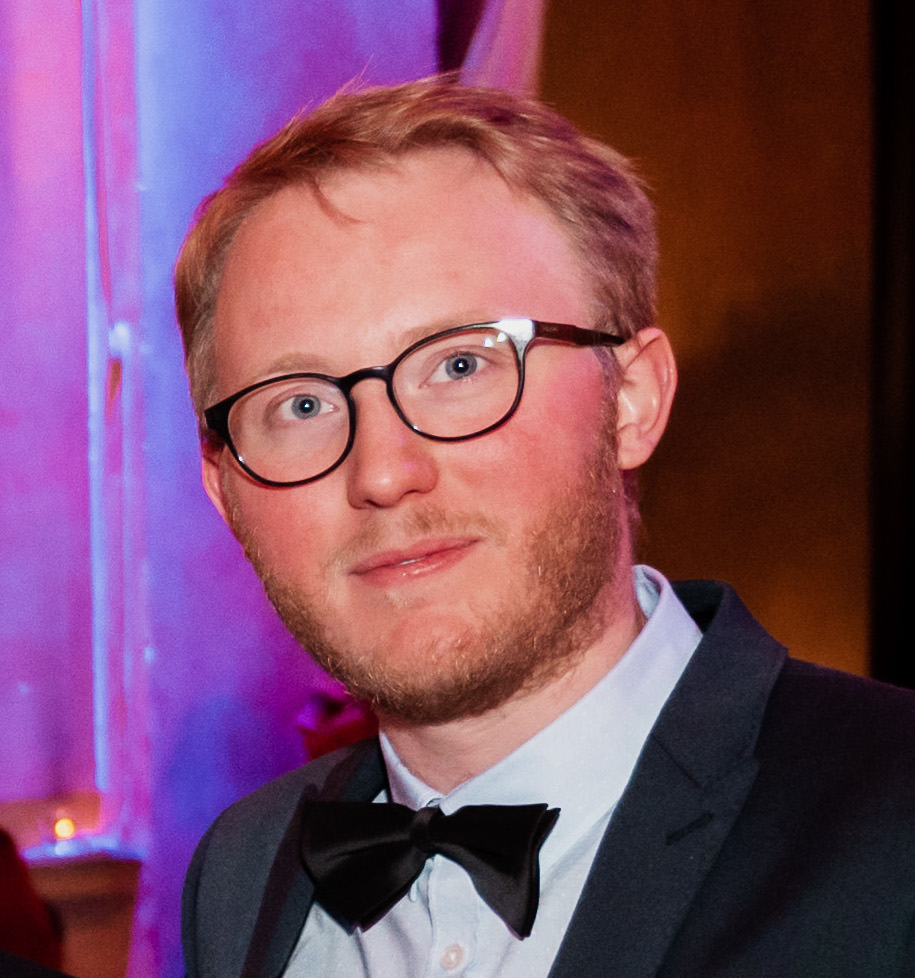
\includegraphics[scale=0.08]{face_pic_3.jpg}

%%%%%%%%%%%%%%%%%%%%%%%%%%%%%%%%%%%%%%
%
%     COLUMN ONE
%
%%%%%%%%%%%%%%%%%%%%%%%%%%%%%%%%%%%%%%

\begin{minipage}[t]{0.33\textwidth} 

%%%%%%%%%%%%%%%%%%%%%%%%%%%%%%%%%%%%%%
%     EDUCATION
%%%%%%%%%%%%%%%%%%%%%%%%%%%%%%%%%%%%%%

\section{Education} 

\subsection{UCLouvain}
\descript{MS in Computer Engineering}
\location{Grad. 2021 | Louvain-la-Neuve, Belgium}
Louvain School of Engineering \\
Major: Networks \& Security \\
\textit{Magna Cum Laude} \\
\location{Cum. GPA: 17.52 / 20}
\sectionsep

\subsection{UCLouvain}
\descript{BS in Engineering}
\location{Grad. 2019 | Louvain-la-Neuve, Belgium}
Louvain School of Engineering \\
Major: Computer Science \\
Minor: Electrical Engineering \\
\textit{Cum Laude} \\
\location{Cum. GPA: 16}
\sectionsep

\subsection{Institut Saint-Joseph}
\location{Grad. 2016 | Ciney, Belgium}
\sectionsep

%%%%%%%%%%%%%%%%%%%%%%%%%%%%%%%%%%%%%%
%     LINKS
%%%%%%%%%%%%%%%%%%%%%%%%%%%%%%%%%%%%%%

\section{Links} 
LinkedIn://  \href{https://www.linkedin.com/in/françois-de-keersmaeker-11301a210/}{\bf François De Keersmaeker} \\
Github:// \href{https://github.com/fdekeers}{\bf fdekeers} \\
Scholar:// \href{https://scholar.google.com/citations?user=UrEkeo4AAAAJ&hl=fr}{\bf François De Keersmaeker} \\
ResearchGate:// \href{https://www.researchgate.net/profile/Francois-De-Keersmaeker}{\bf François De Keersmaeker} \\
ORCID:// \href{https://orcid.org/0000-0002-4967-4132}{\bf 0000-0002-4967-4132}
%Facebook:// \href{https://www.facebook.com/francois.dekeersmaeker.7/}{\bf François De Keersmaeker} \\
%YouTube://  \href{https://www.youtube.com/user/DeedyDash007}{\bf DeedyDash007} \\
%Twitter://  \href{https://twitter.com/debarghya_das}{\bf @debarghya\_das} \\
%Quora://  \href{https://www.quora.com/Debarghya-Das}{\bf Debarghya-Das}

%%%%%%%%%%%%%%%%%%%%%%%%%%%%%%%%%%%%%%
%     COURSEWORK
%%%%%%%%%%%%%%%%%%%%%%%%%%%%%%%%%%%%%%

% \section{Coursework}
% \subsection{Graduate}
% Advanced Machine Learning \\
% Open Source Software Engineering \\
% Advanced Interactive Graphics \\
% Compilers + Practicum \\
% Cloud Computing \\
% Evolutionary Computation \\
% Defending Computer Networks \\
% Machine Learning \\
% \sectionsep

% \subsection{Undergraduate}
% Information Retrieval \\
% Operating Systems \\
% Artificial Intelligence + Practicum \\
% Functional Programming \\
% Computer Graphics + Practicum \\
% {\footnotesize \textit{\textbf{(Research Asst. \& Teaching Asst 2x) }}} \\
% Unix Tools and Scripting \\

%%%%%%%%%%%%%%%%%%%%%%%%%%%%%%%%%%%%%%
%     SKILLS
%%%%%%%%%%%%%%%%%%%%%%%%%%%%%%%%%%%%%%

\section{Skills}
\subsection{Programming}
Shell \textbullet{} Assembly \textbullet{} C \textbullet{} C++ \textbullet{} Java \\
Python \textbullet{} Ruby \textbullet{} Scala \textbullet{} JavaScript \\
Android \textbullet{} Matlab \textbullet{} \LaTeX \textbullet{} Erlang

\subsection{Tools}
SQL \textbullet{} Docker \textbullet{} GDB \textbullet{} Jinja \textbullet{} Arduino \\
Ghidra

% \subsection{Desktop}
% Word \textbullet{} Excel \textbullet{} PowerPoint


\sectionsep

%%%%%%%%%%%%%%%%%%%%%%%%%%%%%%%%%%%%%%
%
%     COLUMN TWO
%
%%%%%%%%%%%%%%%%%%%%%%%%%%%%%%%%%%%%%%

\end{minipage} 
\hfill
\begin{minipage}[t]{0.66\textwidth} 

%%%%%%%%%%%%%%%%%%%%%%%%%%%%%%%%%%%%%%
%     EXPERIENCE
%%%%%%%%%%%%%%%%%%%%%%%%%%%%%%%%%%%%%%

\section{Experience}
\runsubsection{Facebook}
\descript{| Software Engineer }
\location{Jan 2015 - Present | New York, NY}
\sectionsep

\runsubsection{Coursera}
\descript{| KPCB Fellow + Software Engineering Intern }
\location{June 2014 – Sep 2014 | Mountain View, CA}
\vspace{\topsep} % Hacky fix for awkward extra vertical space
\begin{tightemize}
\item 52 out of 2500 applicants chosen to be a KPCB Fellow 2014.
\item Led and shipped Yoda - the admin interface for the new Phoenix platform. 
\item Full-stack developer - Wrote and reviewed code for JS using Backbone, Jade, Stylus and Require and Scala using Play
\end{tightemize}
\sectionsep

\runsubsection{Google}
\descript{| Software Engineering Intern }
\location{May 2013 – Aug 2013 | Mountain View, CA}
\begin{tightemize}
\item Worked on the YouTube Captions team, in Javascript and Python to plan, to design and develop the full stack to add and edit Automatic Speech Recognition captions. In production.
\item Created a backbone.js-like framework for the Captions editor.
\end{tightemize}
\sectionsep

\runsubsection{Phabricator}
\descript{| Open Source Contributor \& Team Leader}
\location{Jan 2013 – May 2013 | Palo Alto, CA \& Ithaca, NY}
\begin{tightemize}
\item Phabricator is used daily by Facebook, Dropbox, Quora, Asana and more.
\item I created the Meme generator and more in PHP and Shell.
\item Led a team from MIT, Cornell, IC London and UHelsinki for the project.
\end{tightemize}
\sectionsep

%%%%%%%%%%%%%%%%%%%%%%%%%%%%%%%%%%%%%%
%     RESEARCH
%%%%%%%%%%%%%%%%%%%%%%%%%%%%%%%%%%%%%%

\section{Research}
\runsubsection{Cornell Robot Learning Lab}
\descript{| Researcher}
\location{Jan 2014 – Jan 2015 | Ithaca, NY}
Worked with \textbf{\href{http://www.cs.cornell.edu/~ashesh/}{Ashesh Jain}} and \textbf{\href{http://www.cs.cornell.edu/~asaxena/}{Prof Ashutosh Saxena}} to create \textbf{PlanIt}, a tool which  learns from large scale user preference feedback to plan robot trajectories in human environments.  
\sectionsep

\runsubsection{Cornell Phonetics Lab}
\descript{| Head Undergraduate Researcher}
\location{Mar 2012 – May 2013 | Ithaca, NY}
Led the development of \textbf{QuickTongue}, the first ever breakthrough tongue-controlled game with \textbf{\href{http://conf.ling.cornell.edu/~tilsen/}{Prof Sam Tilsen}} to aid in Linguistics research. 
\sectionsep

%%%%%%%%%%%%%%%%%%%%%%%%%%%%%%%%%%%%%%
%     AWARDS
%%%%%%%%%%%%%%%%%%%%%%%%%%%%%%%%%%%%%%

\section{Awards} 
\begin{tabular}{rll}
2014	     & top 52/2500  & KPCB Engineering Fellow\\
2014	     & 1\textsuperscript{st}/50  & Microsoft Coding Competition, Cornell\\
2013	     & National  & Jump Trading Challenge Finalist\\
2013     & 7\textsuperscript{th}/120 & CS 3410 Cache Race Bot Tournament  \\
2012     & 2\textsuperscript{nd}/150 & CS 3110 Biannual Intra-Class Bot Tournament \\
2011     & National & Indian National Mathematics Olympiad (INMO) Finalist \\
\end{tabular}
\sectionsep

%%%%%%%%%%%%%%%%%%%%%%%%%%%%%%%%%%%%%%
%     PUBLICATIONS
%%%%%%%%%%%%%%%%%%%%%%%%%%%%%%%%%%%%%%

\section{Publications} 
\renewcommand\refname{\vskip -1.5cm} % Couldn't get this working from the .cls file
\bibliographystyle{abbrv}
\bibliography{publications}
\nocite{*}

\end{minipage} 
\end{document}  \documentclass[]{article}
